\section{Simulation}

A realistic model of the LTCC has been developed, describing the location and material composition
of the support box, the mirrors, photo-multipliers, Winston Cones, magnetic shields and the $C_4F_{10}$ gas.

A 3D view of the simulated geometry of the LTCC \F{simOverview}. The LTCC GEMC simulation software details are summarized in the simulation article of this volume.


\begin{figure}
	\centering
	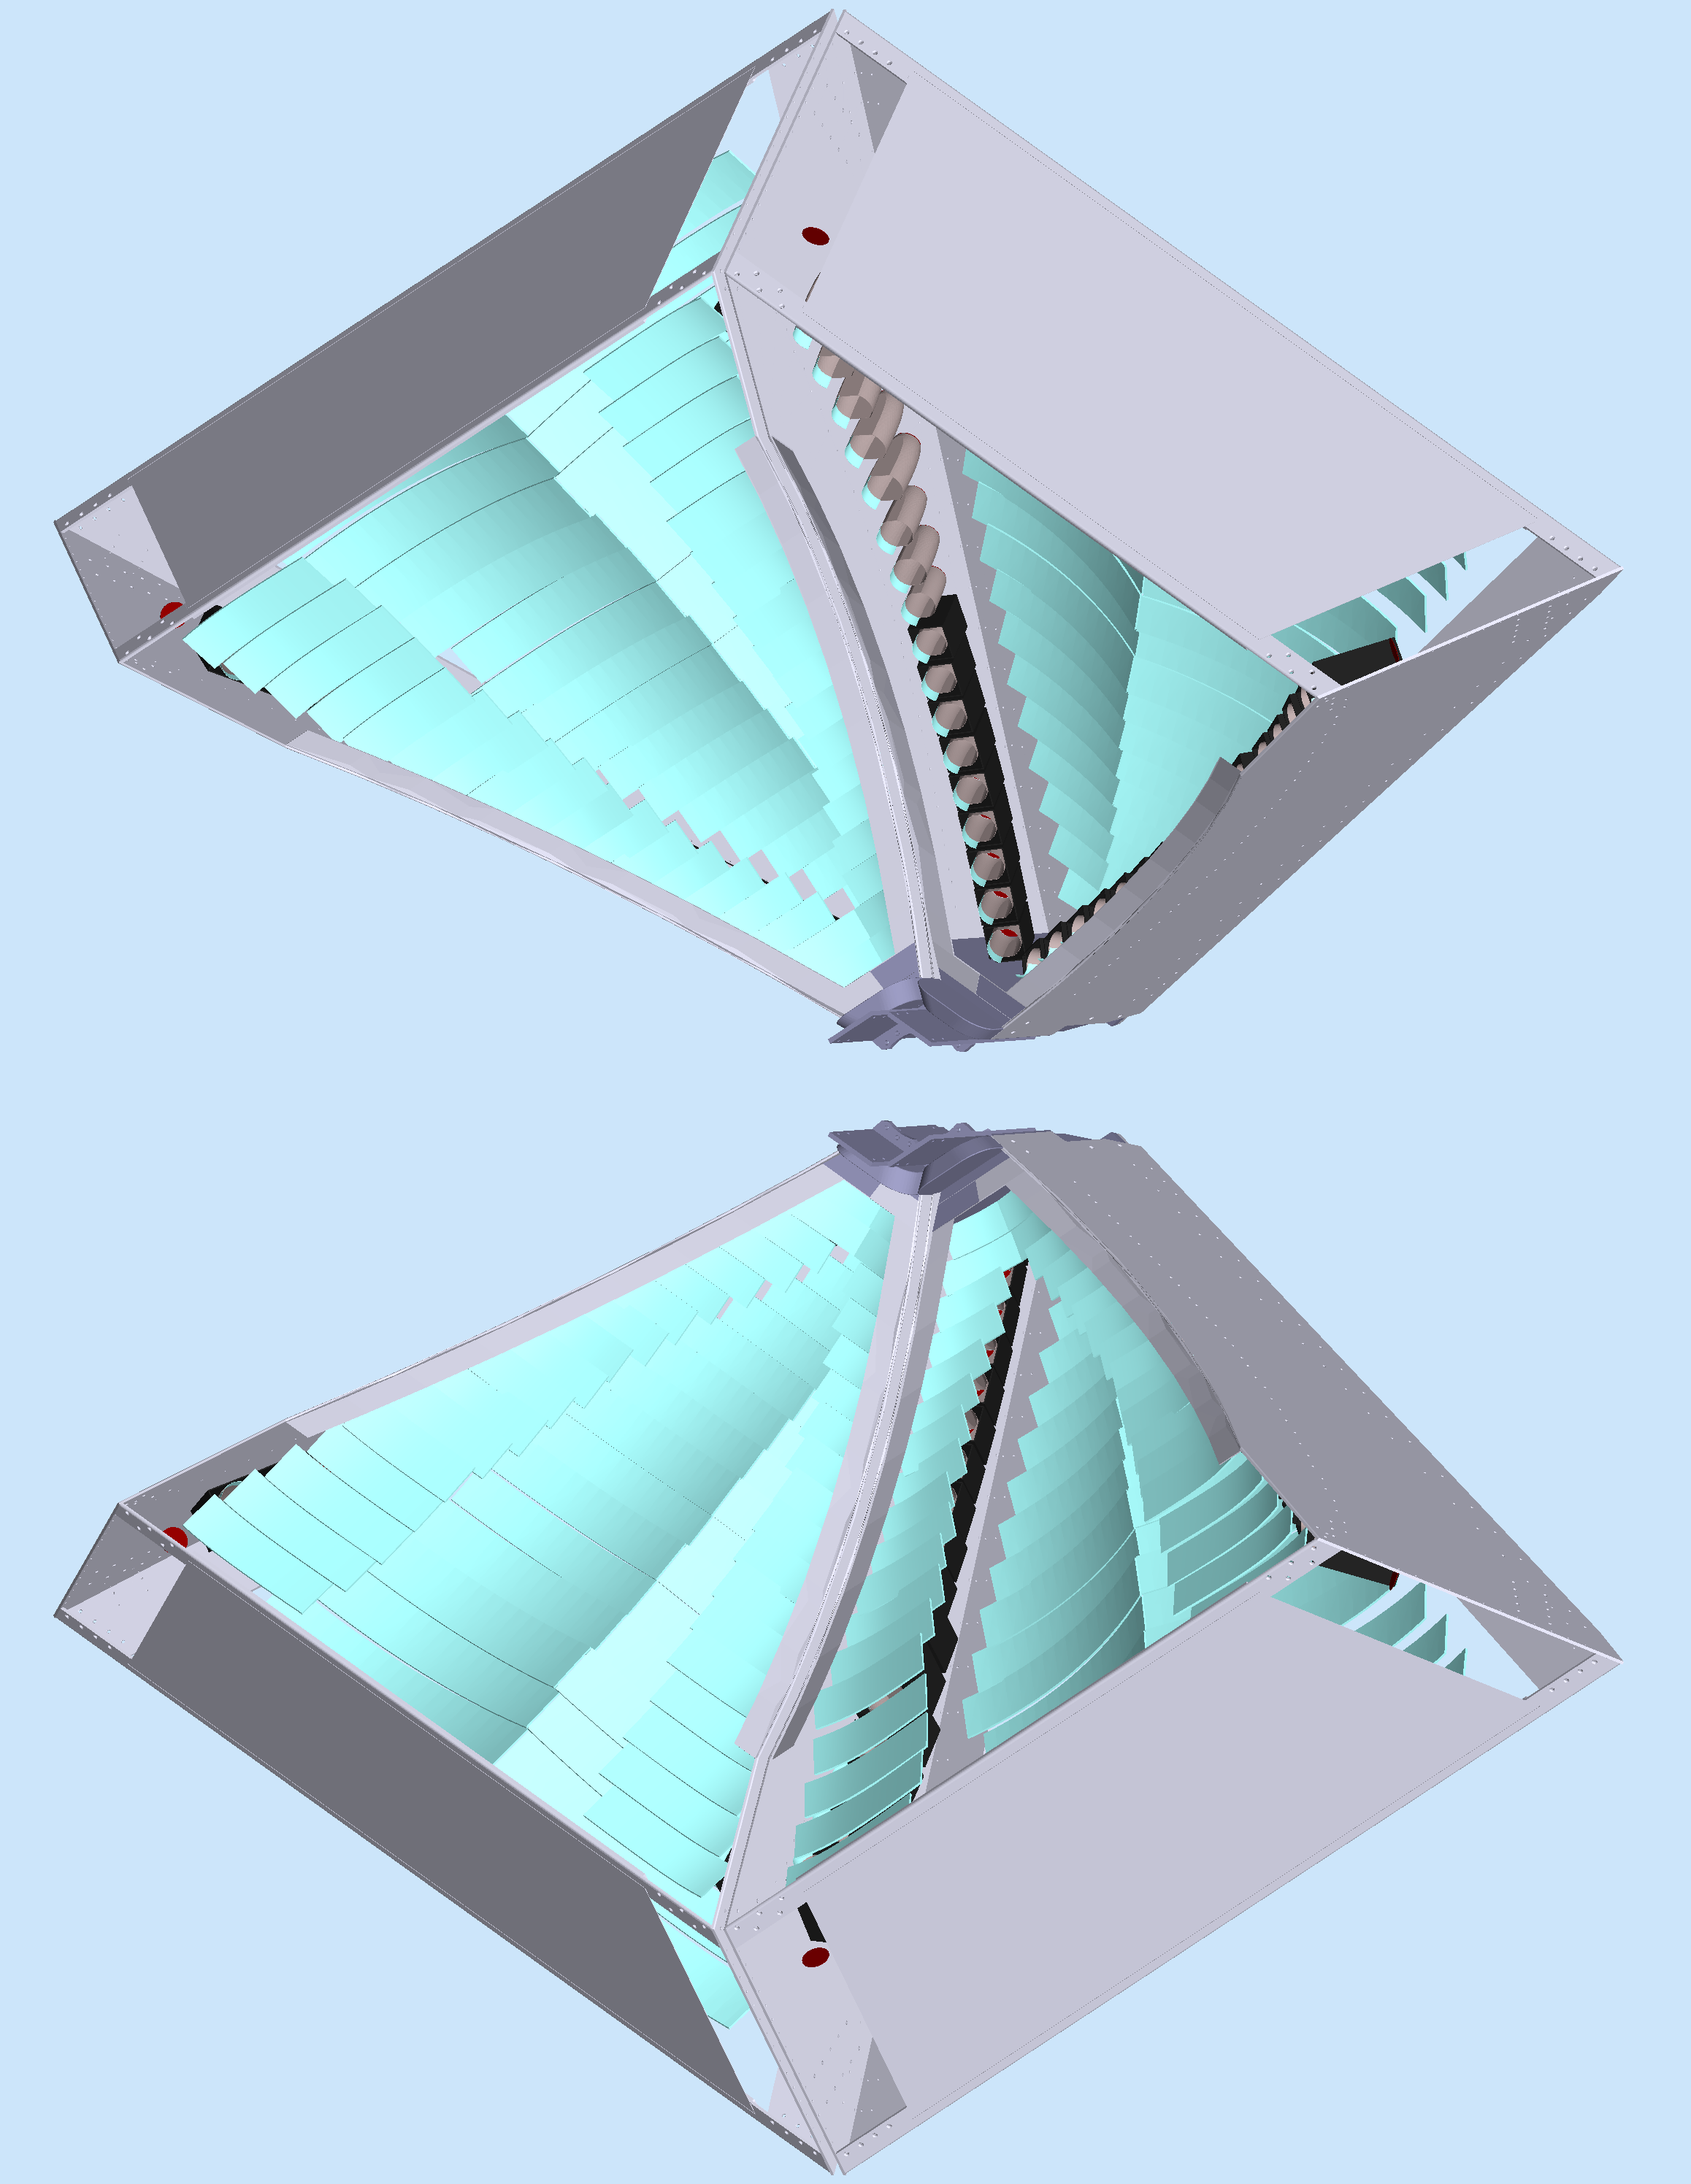
\includegraphics[width=0.95\columnwidth,keepaspectratio]{img/simOverview.png}
	\caption{The geant4 model of the LTCC implemented in GEMC. This view correspond to the Run Group A CLAS12 experiments
				where the LTCC sectors 2, 3, 5 and 6 were present. In this picture the hyperbolic mirrors and some magnetic shields
            in sector3 (upper right) have been made transparent to show details of the Winston Cones (grey) and magnetic shields (black).}
	\label{fig:simOverview}
\end{figure}

\subsection{Geometry}

The Cherenkov light is emitted on a small cone on the same direction of the emitting particle, thus the optics of the LTCC was
designed to maximize the collection of optical photons for both positive and negative particles by considering
optical photons originating from the target (placed on the center of the CLAS12 coordinate system).

The mirror shapes are described mathematically by ellipsoid and hyperbolic curves.
The ellipsoid first focal point is the target location. The second focal point was chosen
to optimize the mirror locations and it overlaps with the hyperbolic first focal point. The hyperbole shape was optimized to focus

geometry:

mirrors maths
box shifts

winston cones
support structure in active area  + nose
pmts shields

digitization
pmts q.e.
output


variations for run periods



